% !TeX spellcheck = ru_RU
% !TEX root = vkr.tex

\section{Обзор}

\subsection{Терминология}

\textit{Граф} --- это упорядоченная пара $(V, E)$, где $V$ множество вершин, а $E$ множество рёбер, соединяющих вершины.

\textit{Ориентированный граф} --- это упорядоченная пара $(V, E)$, где $V$  множество вершин, а $E \subseteq V \times V$ множество упорядоченных пар вершин, называемых дугами.

\textit{Помеченный граф} --- это упорядоченная пара $(G, \mu)$, где $G = (V, E)$ граф с множеством вершин $V$ и множеством рёбер $E$, и $\mu: E \rightarrow L$ отображение, сопоставляющее каждому ребру $e \in E$ метку из множества~$L$.

\textit{Весовая матрица графа} --- это квадратная матрица $A = (a_{ij})$ порядка $n$, где $n$ количество вершин, и элемент $a_{ij}$ равен весу ребра, соединяющего вершины $i$ и $j$, или значению, указывающему на отсутствие ребра между ними.

\textit{Матрица смежности графа} --- это квадратная матрица $A = (a_{ij})$ порядка $n$, где $n$ количество вершин, и элемент $a_{ij}$ равен 1, если между вершинами $i$ и $j$ есть ребро, и 0, если ребра нет.

Для удобства под матрицей смежности ориентированного графа иногда подразумевают весовую, принимая вес между вершинами за 1, а значение, указывающее на отсутствие ребра, за 0. 

\textit{Дерево} --- это структура данных, состоящая из вершин (узлов), связанных между собой рёбрами (ветвями). Начальный узел структуры называется корневым и не имеет ни одного узла-родителя. Каждый узел дерева (кроме листового) может иметь неограниченное количество узлов-потомков. 

\textit{Бинарное дерево} --- это дерево, каждый узел которого (за исключением корневого) имеет ровно два родителя.

\newpage

\subsection{Представление разреженных структур}

Рассмотрим несколько существующих форматов хранения разре\-жен\-ных матриц. Большинство методов основаны на определённых свойствах конкретных структур, следовательно, степень их эффективности может разительно отличаться. 

\textit{Наивный} способ представления разреженных структур предполагает хранение всех элементов, включая нулевые. Этот подход требует больших затрат памяти и на практике малоэффективен.

\textit{Координатное представление} (\textit{COO}) использует тройки ($i$, $j$, $value$) для представления ненулевых элементов разреженной структуры. Параметры ($i$, $j$) указывают на позицию элемента в матрице, а $value$ --- на его значение. На практике используют три неупорядоченных массива (один для каждой координаты тройки) и скаляр, отвечающий за общее количество непустых ячеек \cite{stanimirovic2009performance}. Такая модель используется для хранения небольших разреженных структур и может быть неэффективна при работе с большими данными. В частности, из-за необходимости перебора большого количества троек при поиске, и трудностей с добавлением новых элементов.

Форматы хранения \textit{Compressed Sparse Row} (\textit{CSR}) и \textit{Compressed Spar\-se Column} (\textit{CSC}) не основаны на каком-либо конкретном свойстве
и могут быть использованы для хранения любой разреженной матрицы \cite{stanimirovic2009performance}. Исходные данные распределяются на несколько массивов --- один, содержащий значения ненулевых элементов, один для хранения индексов строк или столбцов (в CSR по строкам, а в CSC по столбцам) соответствующих элементов и один массив-указатель на первое ненулевое вхождение каждой строки или столбца. Аналогично координатному формату вставка или удаление элементов в CSR/CSC может потребовать перестройки всей структуры. Кроме того, в них сложнее обеспечить эффективное параллельное выполнение операций \cite{bulucc2009parallel}.

\textit{Дерево квадрантов} --- это структура данных, часто используемая для представления разреженных двумерных данных. \textit{Q-Tree} разбивается на четыре части (реже на любое другое количество частей), называемых \textit{квадрантами}, где каждый квадрант может быть разбит на четыре подквадранта и т.~д. Если в одной области наблюдаются только элементы одного типа (например, нули в разреженных матрицах), дерево \enquote{обрезают} до одного листа, содержащего информацию об узлах, расположенных на нижних уровнях. При поиске значения в Q-Tree необходимо пройти по дереву, начиная от самого корня. Этот процесс может занимать достаточно много времени, особенно в случаях, когда большое количество данных сосредоточенно в одной области. Но несмотря на другие особенности формата дерево квадрантов удобно использовать для параллельных вычислений.

\subsection{Алгоритм обхода графа в ширину}

Приведём неформальное описание работы алгоритма обхода графа в ширину:

\begin{enumerate}
    \item Инициализировать очередь --- структуру данных для хранения вершин, которые необходимо посетить --- и пустой массив для хранения посещённых вершин. Добавить вершину(-ы), с которой(-ых) начинается поиск, в очередь.
    \item Удалить первую вершину из очереди. Пометить эту вершину как посещённую.
    \item Добавить вершины, которые соединены ребром с текущей, в очередь.
    \item Повторить пункты 2--3, пока очередь не окажется пустой.
\end{enumerate}

Как было упомянуто раннее, линейная алгебра может быть полезна при реализации некоторых этапов BFS, например, для эффективного представления графа или для выполнения операций над матрицами и векторами внутри алгоритма. Далее рассмотрим реализацию шагов 1--4 с использованием векторно-матричных операций. На рис. \ref{fig:bfs} представлен пример работы этого алгоритма:

\begin{figure}
    \centering
    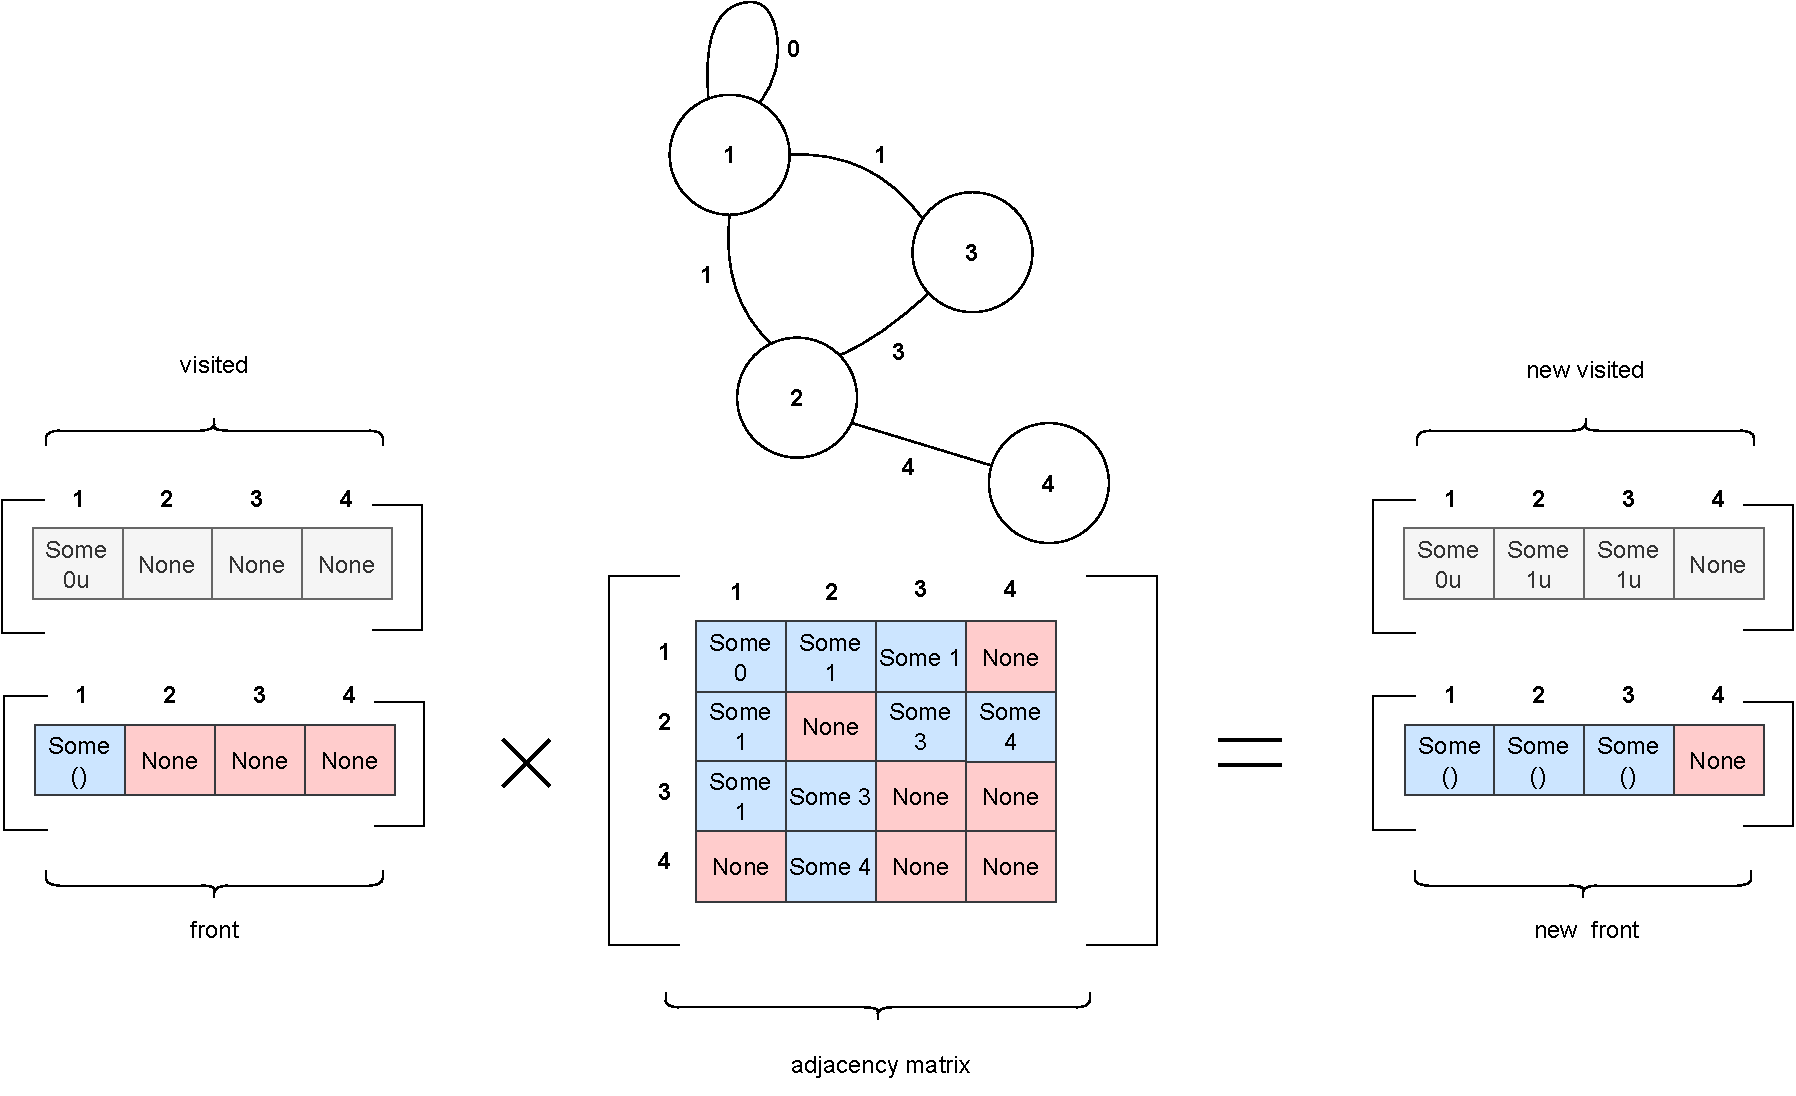
\includegraphics[width=\textwidth]{BFSLinearAlgebra.pdf}
    \caption{Шаги 3--4 BFS с использованием линейной алгебры}
    \label{fig:bfs}
\end{figure}

\begin{enumerate}
    \item Инициализировать матрицу смежности графа (\texttt{ad\-ja\-cen\-cy mat\-rix}), вектор для хранения посещённых вершин (\texttt{visited}) и вектор схожий с очередью, называемый фронтом (\texttt{front}), в котором хранятся вершины, находящиеся на текущем уровне обхода. Добавить вершину(-ы), с которой(-ых) начинается поиск, в \texttt{visited}.
    \item Умножить \texttt{front} на \texttt{adjacency matrix} и получить новый фронт  (\texttt{new front}), добавив, таким образом, все вершины, соединённые с текущей. 
    \item Сложить \texttt{new front} с \texttt{visited} и получить новый вектор (\texttt{mask}) так, что значения из нового фронта \enquote{сохраняются}, только когда они не были помечены в \texttt{visited} (это действие избавит нас от многократного посещения одной и той же вершины). Обновить \texttt{visited} (\texttt{new visited}), используя полученный вектор и векторные операции.
    \item Повторить шаги 2--3, пока все вершины не будут помечены как посещённые.
\end{enumerate}

\subsection{Параллельные вычисления и многопоточность}

Большинство несложных программ, с большой вероятностью выполняются в одном \textit{потоке} (\textit{thread}). Другими словами, в любой момент времени только один оператор находится в процессе выполнения; и если поток блокируется, то вся работа программы останавливается \cite{sarcar2022threading}.

Использование \textit{ядер} центрального процессора может уменьшить общее время простоя и повысить эффективность программы. Как правило, одно ядро за раз \enquote{обслуживает} только один поток. Однако, даже процессор одноядерной машины, быстро переключаясь между задачами, способен создавать иллюзию их одновременного выполнения. В связи с этим, когда несколько потоков, работающих на одном ядре, могут \enquote{чередоваться}, эффективно использовать больше потоков, чем имеющихся ядер \cite{Lee2020}.

При реализации многопоточности необходимо учитывать следующие аспекты:
\begin{enumerate}
    \item \textit{Накладные расходы на синхронизацию}. Во избежание некорректной работы при использовании нескольких потоков необходимо обеспечить их синхронизацию. Координация, в свою очередь, вызывает накладные расходы, что не лучшим образом влияет на производительность.
    \item \textit{Конкуренция за ресурсы}. Когда несколько потоков пытаются получить доступ к общим ресурсам, возникает конкуренция, замедляющая работу программы.
    \item \textit{Накладные расходы на создание}. Создание потоков и управление ими требуют дополнительные ресурсы.
    \item \textit{Зависимость от алгоритмов и данных}. Некоторые алгоритмы (данные) не могут быть эффективно распараллелены из-за своей природы (например, если операция зависит от результата предыдущего шага).
    \item \textit{Зависимость от аппаратного обеспечения}. Некоторые системы имеют ограничения на количество доступных ядер, что ограничивает возможности параллельных вычислений.
\end{enumerate}


